Soit $(Z_{i})= _{i=1,....,N}$ une suite de variables i.i.d telles que $Z_{i}$ suit une loi normale standard $\mathcal{N}(0,1)$ donc de moyenne 0 et variance 1. On va simuler N valeurs (1000 pour la première partie et  on ira jusqu'à 1000000 de tirages) du sous-jacent en simulant un mouvement Brownien. D'où : \[S_{t}(i)=S_{0}e^{(r-\frac{\sigma^{2}}{2})T+\sigma\sqrt{T}Z_{i}}\]

Or, le prix du {\slshape CALL} européen avec la méthode de Monte Carlo est l'espérance qui grace à la loi des grands nombres est:
\[C_{MC}=\frac{1}{N}\sum_{i=1}^{N} (S_{T}(i)-K)_{+}\]

\subsection{Analyse du CALL et du PUT} % (fold)
\label{sub:analyse_du_call_et_du_put}

On présente dans cette section l'approximation du prix du $CALL$ ou du $PUT$ à partir de la simulation d'un mouvement Brownien avec la méthode
 de Monte-Carlo, la fonction permettant de le calculer est Listing~\ref{listing:9} (L'implémentation se trouve dans le fichier \textsc{montecarlo.py}). Les Figure~\ref{fig:call_euro_mc}, et Figure~\ref{fig:put_euro_mc} on observe que la vitesse de convergence est
   plus lente. En effet l'amplitude des oscillations est élevée même après un nombre de tirages dépassant 1 million. De plus, on a implementé
    une fonction qui donne une mesure de la vitesse de convergence de notre méthode (\textsc{v$\_$convergence()}), et cette dernière indique une
	 valeur de $k=\frac{U_n-\text{prix théorique}}{U_{n-1}-\text{prix théorique}}  \neq 0$, avec n grand et des résultats moyénnés sur plusieurs lancements de la  fonction.

De plus on on a tracé deux droites, représentant le rayon de convergence que devrait avoir notre méthode. Sachant que la méthode de Monte-Carlo est une aproximation en $O(\frac{1}{\sqrt(n)})$. Il est intéressant d'analyser le fait qu'en réalisant un développement limité des variations, on acumule une erreur trop importante. La fonction qui implemente cette a était laissé avec le label optionnel et non efficient dans le fichier \textsc{montecarlo.py}.


\begin{figure}[H]
\centering
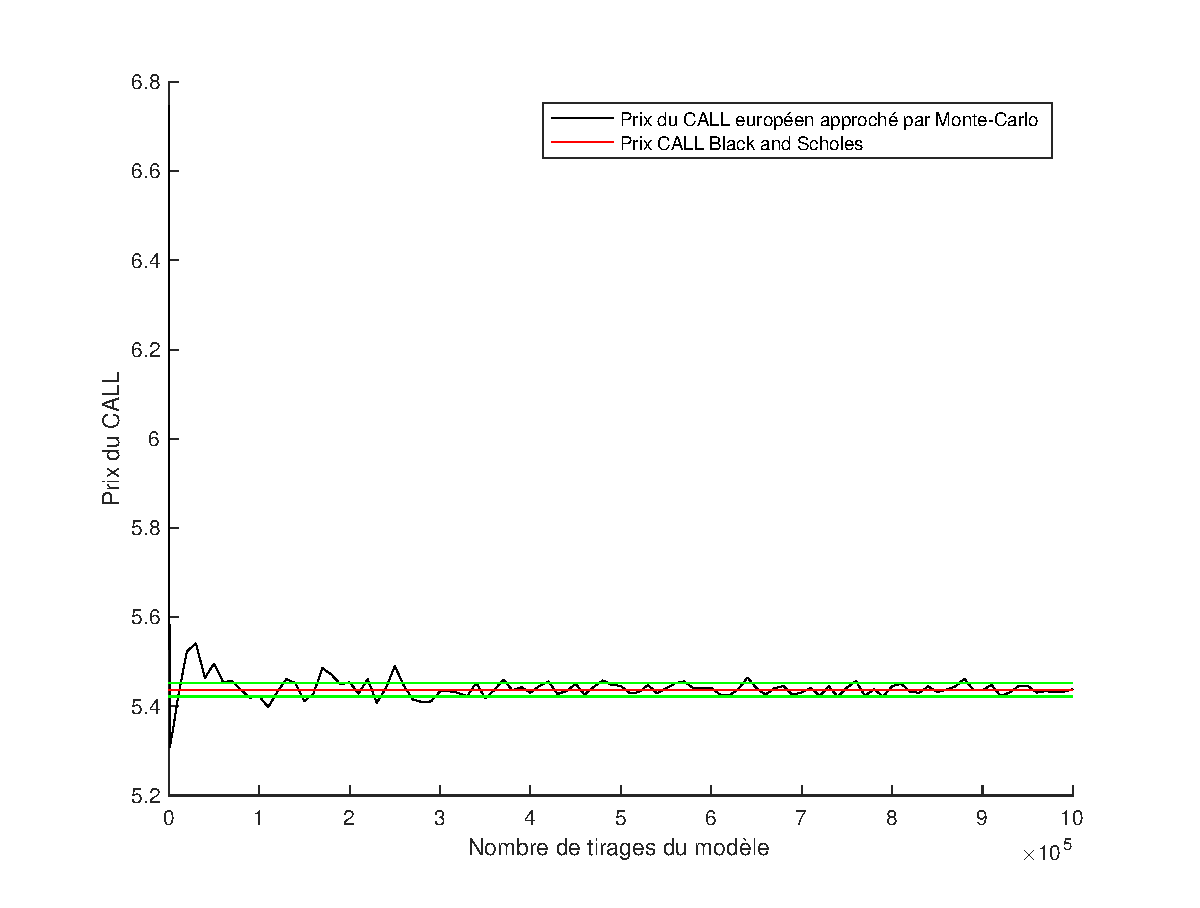
\includegraphics[scale=0.6]{./img/CALL_EURO_MC-BS.eps}
\caption{Variation du prix du CALL européen approché par la méthode de Monte-Carlo en fonction du nombre de tirages}
\label{fig:call_euro_mc}
\end{figure}

\begin{figure}[H]
\centering
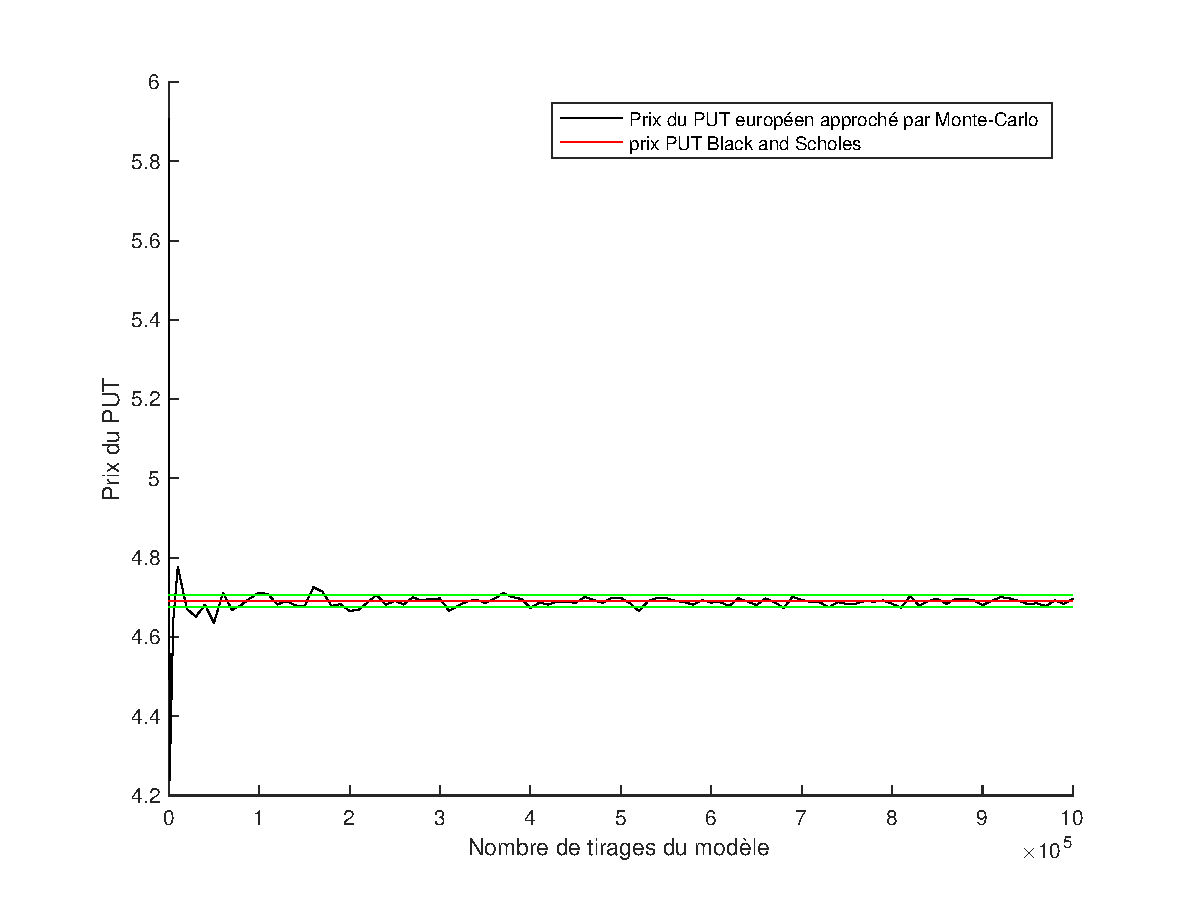
\includegraphics[scale=0.6]{./img/PUT_EURO_MC-BS.eps}
\caption{Variation du prix du PUT européen approché par la méthode de Monte-Carlo en fonction du nombre de tirages}
\label{fig:put_euro_mc}
\end{figure}

% subsection analyse_du_call_et_du_put (end)

\subsection{Analyse pour le delta} % (fold)
\label{sub:analyse_pour_le_delta}

Pour ce qui est du $\delta$ on obtiens des résultats similaires en terme de convergence et de vitesse de convergence. Les variations et leur amplitude sont identiques, seulement les échelles peuvent varier en raison des fortes variances dans les faibles nombres de tirages. La fonction qui permet d'obtenir les résultats est Listing~\ref{listing:6}, et on peut la tester dans le fichier \textsc{delta.py}.

\begin{figure}[H]
\centering
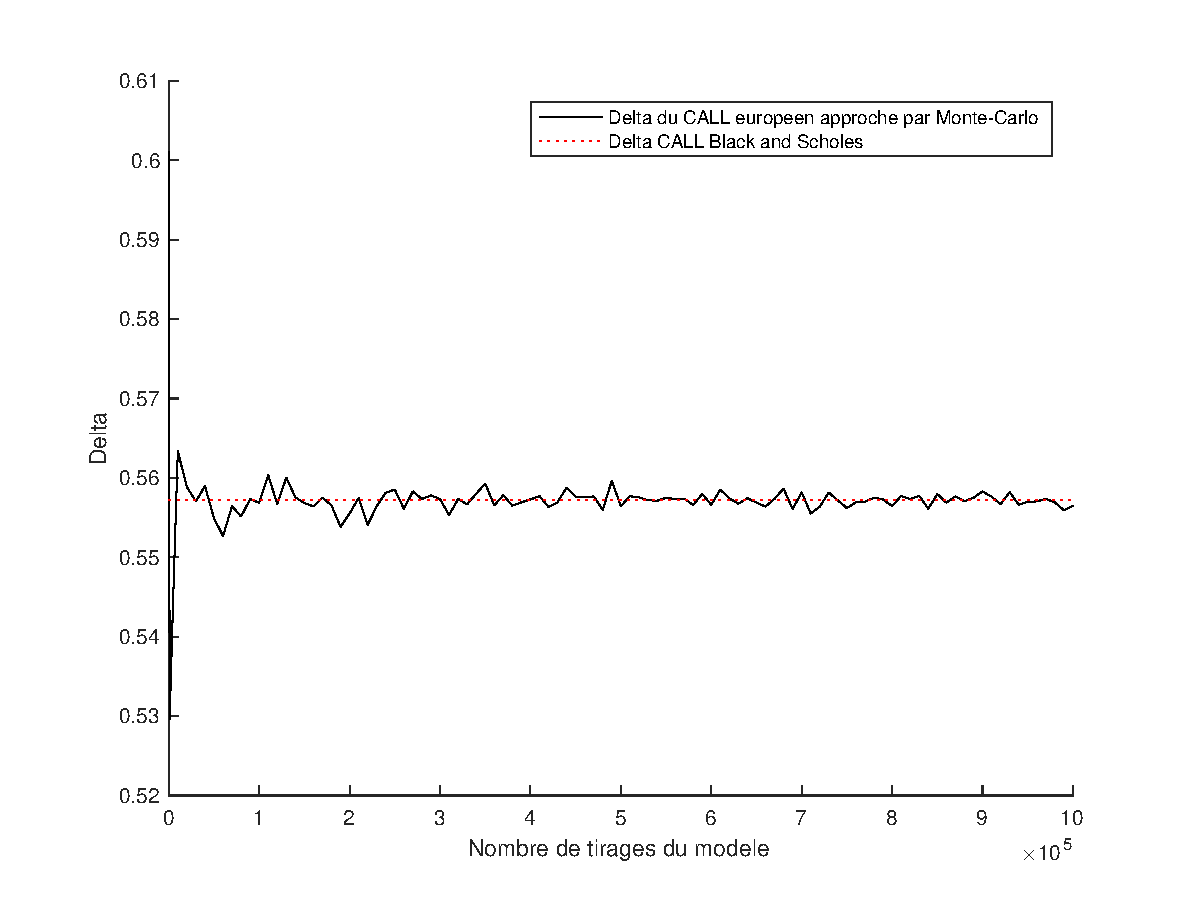
\includegraphics[scale=0.5]{./img/DELTA_CALL_EURO-BS.eps}
\caption{Variation du $\delta$ d'un CALL européen approché par la méthode de Monte-Carlo en fonction du nombre de tirages}
\label{fig:delta_call_euro_mc}
\end{figure}

\begin{figure}[H]
\centering
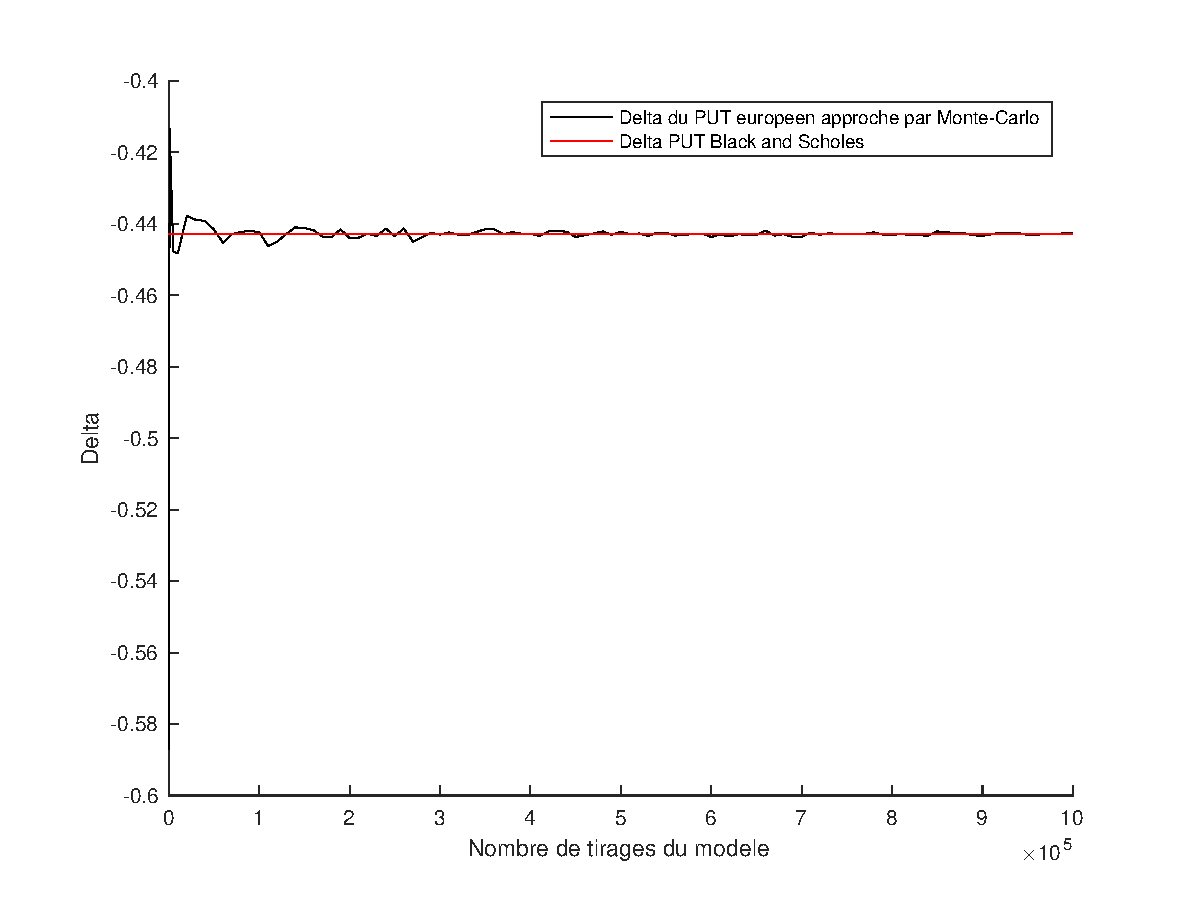
\includegraphics[scale=0.5]{./img/DELTA_PUT_EURO-BS.eps}
\caption{Variation du $\delta$ d'un PUT européen approché par la méthode de Monte-Carlo en fonction du nombre de tirages}
\label{fig:delta_put_euro_mc}
\end{figure}

% subsection analyse_pour_le_delta (end)